\documentclass[dvipdfmx]{jreport}
\usepackage{mypackage}
%%%%%%%%%%%%%%%%%%%%%%%%%%%%%%%%%%
\begin{document}

\chapter{実験装置及び手順}

\section{装置全体図}
\begin{figure}[htbp]
  \begin{center}
    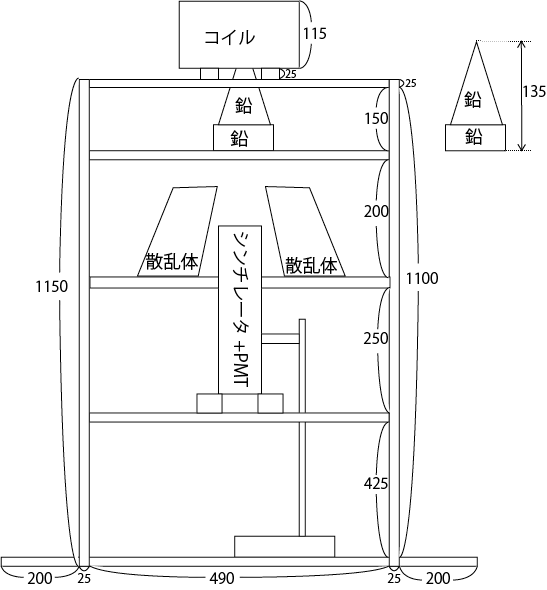
\includegraphics[width=100mm]{figure/setup.png}
    \caption{装置全体図 \label{setup}}
  \end{center}
\end{figure}

\section{各実験装置}

\subsection{シールド}

\subsubsection{鉛シールドによるガンマ線の吸収}
物質中をガンマ線が透過する際に、進んだ長さに対応して強度は減衰する。
物質中に$1$個のガンマ線が入射した際に透過する確率は、吸収係数$\mu\ \mathrm{/cm}$(入射光子のエネルギーに依存)と、物質中を光子が通過する長さ$x\ \mathrm{cm}$を用いて
\begin{equation}
  \label{gensui}
  I = \exp(- \mu x)
\end{equation}
とかける。一般には質量吸収係数$\mu_{m} = \mu / \rho\ \mathrm{cm^{2}/g}$がよく用いられ、これと物質の密度$\rho\ \mathrm{g/cm^3}$用いると
\begin{equation}
  I = \exp(- \mu_{m} \rho x)  
\end{equation}
とかける。ただし、実際に検出器で検出されるガンマ線は、吸収物質を透過したものだけでなく、吸収物質中で散乱されたものも含まれている。
この効果の補正を入れるために式$\ref{gensui}$の係数を以下のようにビルドアップ係数$B\qty(x,E_{\gamma})$で置き換える。
\begin{equation}
  I = B\qty(x,E_{\gamma})\exp(- \mu x)
\end{equation}
ビルドアップ係数は経験則的には、吸収物質の厚さを入射ガンマ線の平均自由行程で割った値にほぼ等しい。
本実験で用いる鉛の場合、$1\mathrm{MeV}$に対応する質量吸収係数が約$6.8 \cdot 10^{-2} \mathrm{cm^{2}/g}$、密度が$11.34 \mathrm{g/cm^{3}}$であるから、式$\ref{mfp}$より鉛中の平均自由行程は
$1.29\mathrm{cm}$であり、経験則的なビルドアップ係数は
\begin{equation}
  B_{\mathrm{experimental}} = \frac{x}{1.29\mathrm{cm}}
\end{equation}
となる。
今回用いるシールドは厚みが$20\mathrm{cm}$のものであり、それに対する透過確率を図$\ref{lead_attenuation}$に示す。
\begin{figure}[htbp]
  \begin{center}
    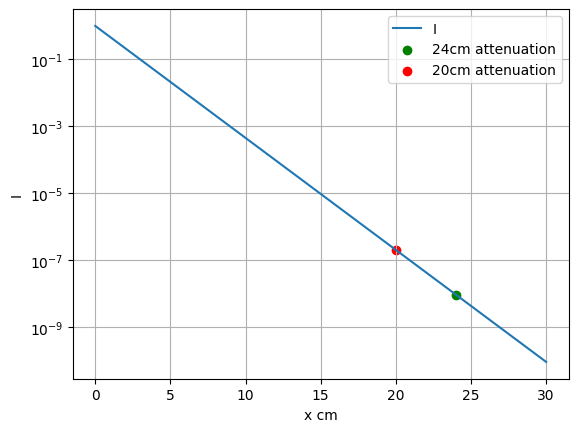
\includegraphics[width=100mm]{figure/lead_attenuation.png}
    \caption{鉛の長さに対する$\gamma$の透過確率 \label{lead_attenuation}}
  \end{center}
\end{figure}

\subsection{散乱体}

\subsubsection{$\ce{Sm_{2}O_{3}}$散乱体におけるガンマ線の平均自由行程}
平均自由行程は
\begin{equation}
  \label{mfp}
  \lambda = \frac{\int_{0}^{\infty} xe^{-\mu x} dx}{\int_{0}^{\infty} e^{-\mu x} dx} = \frac{1}{\mu} = \frac{1}{\mu_{m} \rho}
\end{equation}
とかける。$\mathrm{Sm_{2}O_{3}}$散乱体の密度を$1.7\ \mathrm{g/cm^3}$とした場合の$960\ \mathrm{keV}$のガンマ線の平均自由行程は$9.8\ \mathrm{cm}$である。

\subsubsection{散乱体ケース材質の選定}
ノイズ信号として散乱体ケースによりコンプトン散乱された光子が考えられる。散乱$\gamma$線の微分散乱断面積は、クライン・仁科の式
\begin{equation}
  \dv{\sigma}{\Omega} = Zr_{0}^{2} \qty[\frac{1}{1 + \alpha \qty(1 - \cos \theta)}]^{2} \qty[\frac{1 + \cos^{2} \theta}{2}]
  \qty[1 + \frac{\alpha^{2} \qty(1 - \cos \theta)^{2} }{\qty(1 + \cos^2 \theta) \qty[1 + \alpha \qty(1 - \cos \theta)]}]
\end{equation}
に従う。これは吸収物質の原子番号$Z$に比例するので、なるべくこの値が小さいものを散乱体ケースに採用するのが望ましい。

\subsubsection{散乱体ケースの設計}
% 散乱体ケースを図$\ref{散乱体ケース図面}$のように設計した。
% \begin{figure}[htbp]
%   \centering
%   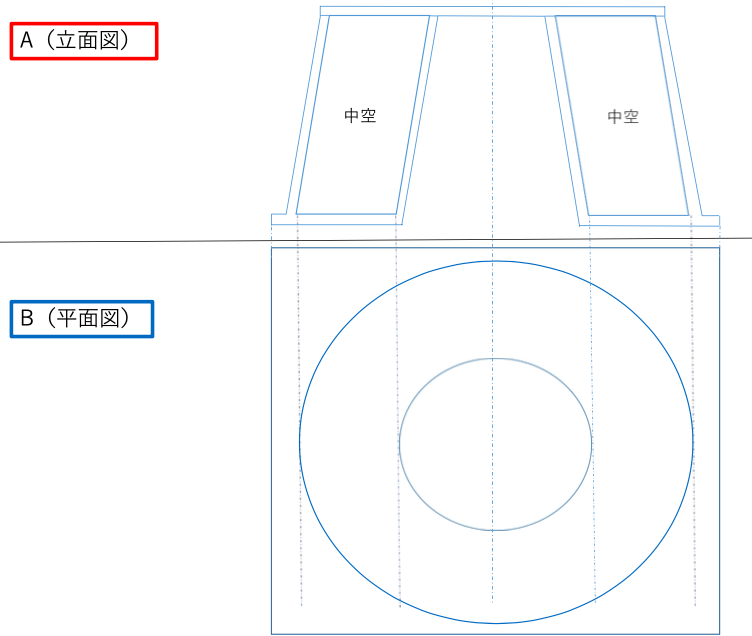
\includegraphics[width=70mm]{sanrantai1.png}
%   \caption{散乱体ケース \label{散乱体ケース}}
% \end{figure}
% \begin{figure}[htbp]
%   \centering
%   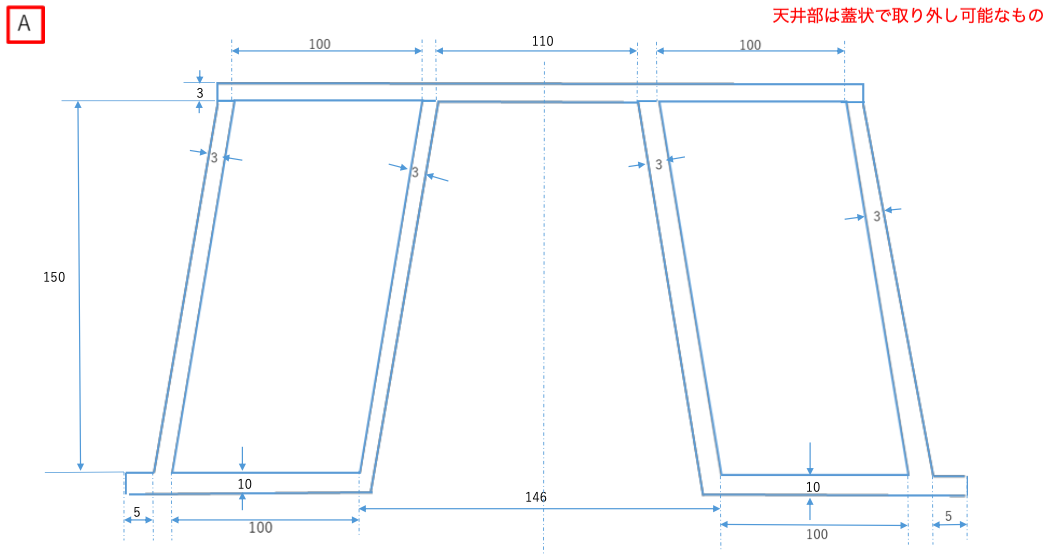
\includegraphics[width=70mm]{sanrantai2.png}
%   \caption{散乱体ケース図面 \label{散乱体ケース図面}}
% \end{figure}

\subsection{検出器}

\subsubsection{$\ce{LaBr_{3}}$シンチレータ}
$\ce{LaBr_{3}}$シンチレータの特徴として
\begin{itemize}
\item 高いエネルギー分解能
\item 短い減衰時間
\item 大きい結晶密度
\end{itemize}
が挙げられる。
減衰時間$26\mathrm{ns}$。

\subsubsection{光電子増倍管}
シンチレータで発生した光子が、光電面に入射することで光電効果により光電子を叩き出す。この光電子が持っているエネルギーは高々$1\mathrm{eV}$程度である。
光電子は増倍部でダイノード間の数$100\mathrm{eV}$程度の電位差によって加速され、ダイノードと衝突し二次電子が放出される。典型的な二次電子の個数は$5$から$10$個程度である。
光電子増倍管の全利得を考える。1個の入射光電子ごとに$\delta$個の電子が生成されるとすると、増倍部が$N$段ある場合、全体での利得は
\begin{equation}
  \mathrm{gain} = \alpha \delta^{N}
\end{equation}
で与えられる。ただし、$\alpha$は増倍部に集められる光電子の割合である。$\delta$は一般的にはダイノード間電圧の1より小さい累乗で変化し、$10$段程度の場合、全利得は$V^{6}$から$V^{9}$に比例する。

\subsubsection{AD変換器}
光電子増倍管からの信号である電圧はアナログ信号であるため、AD変換器を通してデジタル信号に変換する。
本実験で用いるADCはCAEN DT5740である。これは電荷積分型ADCで、GATE信号が入力されている間のみ電荷積分を行う。このGATE信号を作るためにDiscriminatorを用いる。
ADCからの出力波形の面積がエネルギーに対応している。
キャリブレーションを行う際には、この面積を測って、ある面積の波が何個きているか数える。
サンプリングレートは62.5MS/sであり、18ns/Sである。

\subsubsection{エネルギー分解能}

\paragraph{原理}
シンチレータの発光に引き続いて、光電子増倍管の光電陰極から発生する電子の数は統計的にランダムに変動する離散的な数である。このキャリア形成過程がポアソン分布に従うと仮定する。
あるエネルギーの光子が光電子増倍管に入射した際に、平均として$N$個のキャリアが形成されたとすると、その統計的な変動における標準偏差は$\sqrt{N}$になる。
通常、$N$は非常に大きい数なので、エネルギーに対する計数の応答はガウス分布となる。そこで、一般的には分解能$R$はスペクトルの半値幅をピークの中央値$H_{0}$で割ったものとして無次元化されて定義される
\begin{equation}
  R = \frac{\mathrm{FWHM}}{H_{0}} = \frac{2.35\sigma}{H_0}
\end{equation}
形成されるキャリアの数は入射光子のエネルギーに対し線形に応答するので、比例定数を$K$とおいて
\begin{equation}
  H_{0} = KN
\end{equation}
その標準偏差は
\begin{equation}
  \sigma = K\sqrt{N}
\end{equation}
となる。したがってキャリア数の統計的変動による分解能の限界値は以下のようになる。
\begin{equation}
  R_{\mathrm{ポアソン限界}} = \frac{\mathrm{FWHM}}{H_{0}} = \frac{2.35K\sqrt{N}}{KN} = \frac{2.35}{\sqrt{N}}
\end{equation}
実際の検出器の分解能には、個々のキャリアの形成過程が独立でないことによる補正が加わる。この統計的変動のポアソン分布からのずれを以下のファノ因子を用いて表す。
\begin{equation}
  F = \frac{観測されたNの分散}{ポアソン分布で予想された分散\qty(=N)}
\end{equation}
ファノ因子の値は検出器によって異なる。シンチレータではファノ因子は$1$と等しいことが知られている。ファノ因子を用いると分解能の統計限界は
\begin{equation}
  R_{統計限界} = \frac{2.35\sqrt{F}}{\sqrt{N}}
\end{equation}
と求まる。

\paragraph{理論値}
理論的な分解能は以下に示す値によって決定される。
\begin{itemize}
\item $\ce{LaBr_{3}}$シンチレータの絶対発光量(光子/MeV):63000
\item 光電子増倍管の量子効率:0.2〜0.3
\end{itemize}
ただし、量子効率と増倍係数は以下のように定義される。
\begin{equation}
  量子効率\qty(\mathrm{QE}) = \frac{発生する光電子の数}{入射した光子の数}
\end{equation}
したがって$1\mathrm{MeV}$におけるキャリア形成数は10段のPMTを用いたとき
\begin{equation}
  N = 63000 \times 0.2 = 1.26\cdot10^{4}
\end{equation}
であり
\begin{equation}
  \sqrt{N} = 1.1\cdot10^{2}
\end{equation}
なので分解能の統計限界は
\begin{equation}
  R_{統計限界} = \frac{2.35\sqrt{F}}{\sqrt{N}} = 2.0\cdot10^{-2}
\end{equation}
と求まる。

\paragraph{実験値}
今回用いる$\ce{LaBr_{3}}$シンチレータの$841\mathrm{keV}$と$963\mathrm{keV}$における分解能を、表$\ref{caribration}$の値を外挿して求めた。
分解能がキャリア形成数の平方根の逆乗に比例し、キャリア形成数はエネルギーに比例することから、外挿する関数としてエネルギーの平方根の逆乗に比例する関数を選んだ。
その結果を表$\ref{resolution}$に示す。
\begin{table}[hbtp]
  \caption{キャリブレーション \label{caribration}}
  \centering
  \begin{tabular}{ccccc}
    \hline
    核種 & エネルギー & 中心$H_{0}$(channel) & 標準偏差$\sigma$(channel) & 分解能$R$ \\
    \hline \hline
    $\ce{^{22}Na}$ & $511\mathrm{keV}$ & $204.0$ & $8.1$ & $9.3\cdot10^{-2}$\\
    $\ce{^{137}Cs}$ & $662\mathrm{keV}$ & $265.0$ & $9.3$ & $8.3\cdot10^{-2}$\\
    $\ce{^{22}Na}$ & $1275\mathrm{keV}$ & $501.0$ & $14.0$ & $6.6\cdot10^{-2}$\\
    \hline
  \end{tabular}
\end{table}

\begin{table}[hbtp]
  \caption{エネルギー分解能 \label{resolution}}
  \centering
  \begin{tabular}{cccc}
    \hline
    核種 & エネルギー & 分解能$R$ & FWHM(keV)\\
    \hline \hline
    $\ce{^{152\mathrm{m}}Eu}$ & $841\mathrm{keV}$ & $7.4\cdot10^{-2}$ & $62.2$\\
    $\ce{^{152\mathrm{m}}Eu}$ & $963\mathrm{keV}$ & $7.0\cdot10^{-2}$ & $67.4$\\
    \hline
  \end{tabular}
\end{table}

\subsubsection{キャリブレーション}
\begin{figure}[htbp]
  \begin{minipage}[b]{0.45\linewidth}
    \centering
    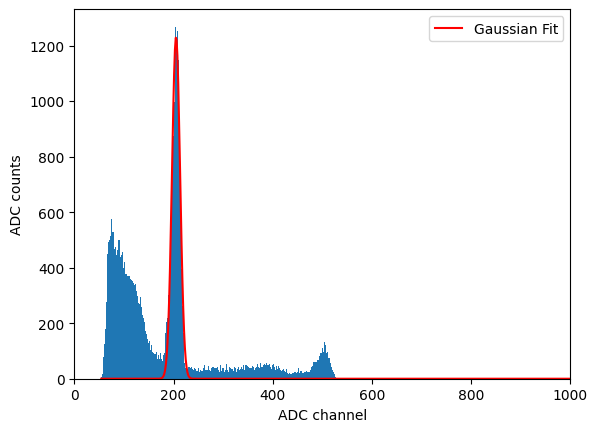
\includegraphics[width=80mm]{figure/Na22_10min_511.png}
    \caption{$\ce{^{22}Na}$ $511\mathrm{keV}$ \label{511}}
  \end{minipage}
  \begin{minipage}[b]{0.45\linewidth}
    \centering
    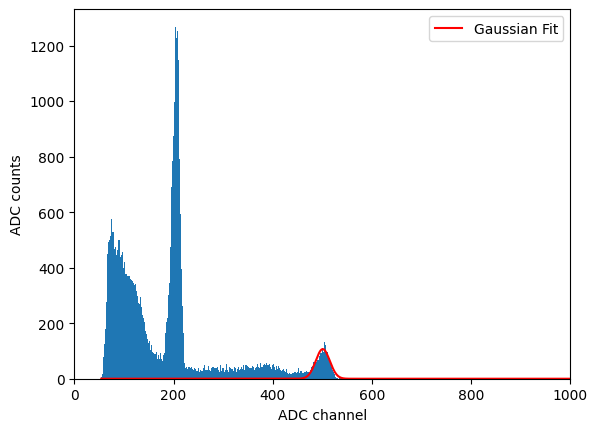
\includegraphics[width=80mm]{figure/Na22_10min_1275.png}
    \caption{$\ce{^{22}Na}$ $1275\mathrm{keV}$ \label{1275}}
  \end{minipage}
\end{figure}
\begin{figure}[htbp]
  \centering
  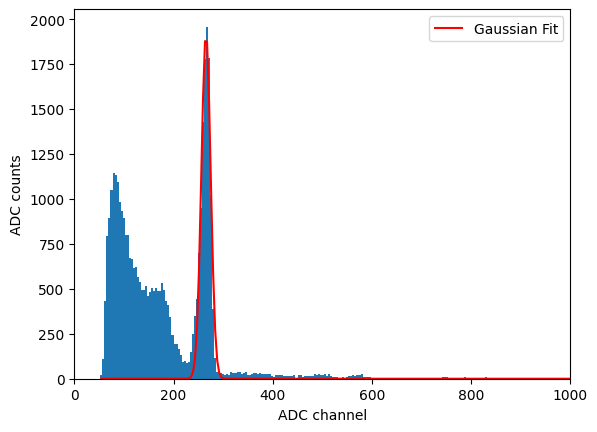
\includegraphics[width=80mm]{figure/Cs137_10min.png}
  \caption{$\ce{^{137}Cs}$ $662\mathrm{keV}$ \label{Cs137}}
\end{figure}
図$\ref{511}$と図$\ref{1275}$に$\ce{^{22}Na}$の波形を示す。また、図$\ref{Cs137}$に$\ce{^{137}Cs}$の波形を示す。
以上より図$\ref{linear_ap}$に示すように線形に外挿すると、今回のセットアップを用いた際のADCのチャネルとエネルギーの関係が
\begin{figure}[htbp]
  \centering
  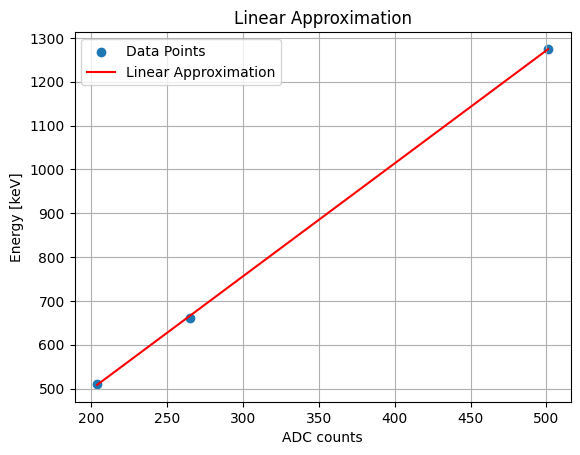
\includegraphics[width=80mm]{figure/linear_ap.png}
  \caption{キャリブレーション\label{linear_ap}}
\end{figure}
\begin{equation}
  \mathrm{Energy\ \ keV} = 2.58 \times \mathrm{channel} - 18.0
\end{equation}
と求まる。

\section{回路}

\subsection{回路全体図}

\begin{figure}[htbp]
  \begin{center}
    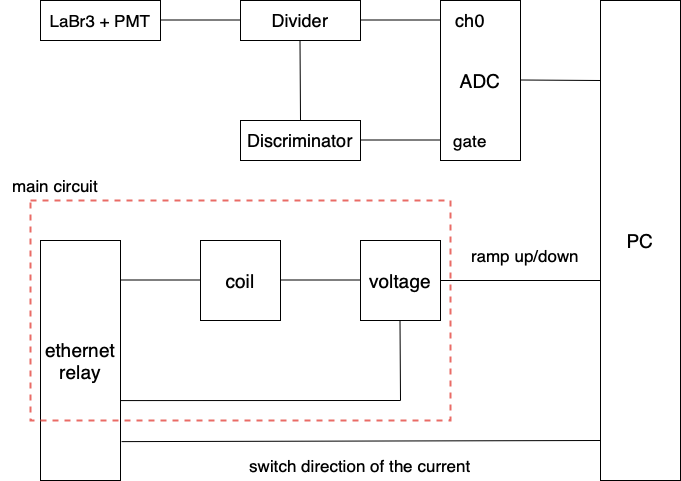
\includegraphics[width=100mm]{figure/overall_circuit.png}
    \caption{回路全体図 \label{overall_circuit}}
  \end{center}
\end{figure}

\subsection{反転回路}
本実験では各回での放射化における放射能の差による誤差をできるだけ少なくするため、短い時間間隔で磁場を反転させる。
反転回路の概略を図$\ref{main_circuit}$に載せる。また、その制御を表$\ref{reverse_signal}$に載せる。10秒のスリープタイムを設け、5分間測定ののち磁場を反転する。
今回の実験では、ds3484イーサネットリレーを用いて反転信号を制御する。

\begin{table}[hbtp]
  \caption{反転信号 \label{reverse_signal}}
  \centering
  \begin{tabular}{ccccc}
    \hline
    \ctext{1} & \ctext{2} & \ctext{3} & \ctext{4} & status\\
    \hline \hline
    0 & 0 & 0 & 0 & off\\
    1 & 0 & 0 & 0 & off\\
    1 & 1 & 0 & 0 & on(down)\\
    1 & 0 & 0 & 0 & off\\
    0 & 0 & 0 & 0 & off\\
    0 & 0 & 1 & 0 & off\\
    0 & 0 & 1 & 1 & on(up)\\
    0 & 0 & 1 & 0 & off\\
    \hline
  \end{tabular}
\end{table}

\begin{figure}[htbp]
   \centering
   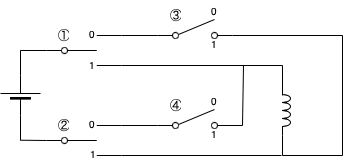
\includegraphics[width=100mm]{figure/main_circuit.png}
   \caption{反転回路 \label{main_circuit}}
\end{figure}

\section{実験手順}

\end{document}
